%%%%%%%%%%%%%%%%%%%%%%%%%%%%%%%%%%%%%%%%%%%%%%%%%%%%%%%%%%%%%%%%%%%%%%%%%%%%
% AGUJournalTemplate.tex: this template file is for articles formatted with LaTeX
%
% This file includes commands and instructions
% given in the order necessary to produce a final output that will
% satisfy AGU requirements, including customized APA reference formatting.
%
% You may copy this file and give it your
% article name, and enter your text.
%
% guidelines and troubleshooting are here:

%% To submit your paper:
\documentclass[draft]{../agujournal2019}
\usepackage{url} %this package should fix any errors with URLs in refs.
\usepackage{lineno}
\usepackage[inline]{../trackchanges} %for better track changes. finalnew option will compile document with changes incorporated.
\usepackage{soul}
\usepackage{amsmath}
\usepackage{pifont}  % 输入带圈数字,参考https://blog.csdn.net/tsingke/article/details/105961016
% \usepackage{xr}
% \usepackage{xr-hyper}
% % 参考其它文件的标签 https://texfaq.org/FAQ-extref
% \externaldocument[SI]{../sup/supplementary_information}
\linenumbers
%%%%%%%
% As of 2018 we recommend use of the TrackChanges package to mark revisions.
% The trackchanges package adds five new LaTeX commands:
%
%  \note[editor]{The note}
%  \annote[editor]{Text to annotate}{The note}
%  \add[editor]{Text to add}
%  \remove[editor]{Text to remove}
%  \change[editor]{Text to remove}{Text to add}
%
% complete documentation is here: http://trackchanges.sourceforge.net/
%%%%%%%

\draftfalse

%% Enter journal name below.
%% Choose from this list of Journals:
%
% JGR: Atmospheres
% JGR: Biogeosciences
% JGR: Earth Surface
% JGR: Oceans
% JGR: Planets
% JGR: Solid Earth
% JGR: Space Physics
% Global Biogeochemical Cycles
% Geophysical Research Letters
% Paleoceanography and Paleoclimatology
% Radio Science
% Reviews of Geophysics
% Tectonics
% Space Weather
% Water Resources Research
% Geochemistry, Geophysics, Geosystems
% Journal of Advances in Modeling Earth Systems (JAMES)
% Earth's Future
% Earth and Space Science
% Geohealth
%
% ie, \journalname{Water Resources Research}

\journalname{Water Resources Research}


\begin{document}
\justify
%%%%%%%%%%%%%%%%%%%%%%%%%%%%%%%%%%%%%%%%%%%%%%%
%  TITLE
%
% (A title should be specific, informative, and brief. Use
% abbreviations only if they are defined in the abstract. Titles that
% start with general keywords then specific terms are optimized in
% searches)
%
%%%%%%%%%%%%%%%%%%%%%%%%%%%%%%%%%%%%%%%%%%%%%%%
%\includegraphics{agu_pubart-white_reduced.eps}

\graphicspath{{/Users/songshgeo/Documents/VSCode/WGRegimes_YRB_2020/figures}}
\title{Identifying regime transitions for water governance at the Yellow River Basin, China}
%
% e.g., \title{Supporting Information for "Terrestrial ring current:
% Origin, formation, and decay $\alpha\beta\Gamma\Delta$"}
%
%DOI: 10.1002/%insert paper number here%

%% ------------------------------------------------------------------------ %%
%
%  AUTHORS AND AFFILIATIONS
%
%% ------------------------------------------------------------------------ %%


% List authors by first name or initial followed by last name and
% separated by commas. Use \affil{} to number affiliations, and
% \thanks{} for author notes.
% Additional author notes should be indicated with \thanks{} (for
% example, for current addresses).

% Example: \authors{A. B. Author\affil{1}\thanks{Current address, Antartica}, B. C. Author\affil{2,3}, and D. E.
% Author\affil{3,4}\thanks{Also funded by Monsanto.}}

\authors{
      Shuang Song\affil{1},
      Shuai Wang\affil{1},
      Xutong Wu\affil{1},
      yongping Wei\affil{2},
      Graeme S. Cumming\affil{3},
      Yue Qin\affil{4},
      Xilin Wu\affil{5},
      Bojie Fu\affil{1,5}
}


\affiliation{1}{
      State Key Laboratory of Earth Surface Processes and Resource Ecology,
      Beijing Normal University,
      Beijing, 100875, Beijing, China.
}
\affiliation{2}{
      School of Earth and Environmental Sciences,
      The University of Queensland,
      Brisbane, 4067, QLD, Australia.
}
\affiliation{3}{
      ARC Centre of Excellence for Coral Reef Studies,
      James Cook University,
      Townsville, 4811, QLD, Australia.
}
\affiliation{4}{
      College of Environmental Sciences and Engineering,
      Peking University,
      Beijing, 100875, Beijing, China.
}
\affiliation{5}{
      State Key Laboratory of Urban and Regional Ecology,
      Research Center for Eco-Environmental Sciences,
      Chinese Academy of Sciences,
      Beijing, 100875, Beijing, China.
}

%(repeat as many times as is necessary)


% Corresponding author mailing address and e-mail address:

% (include name and email addresses of the corresponding author.  More
% than one corresponding author is allowed in this LaTeX file and for
% publication; but only one corresponding author is allowed in our
% editorial system.)

% Example: \correspondingauthor{First and Last Name}{email@address.edu}

\correspondingauthor{Shuai Wang}{shuaiwang@bnu.edu.cn}



%%%%%%%%%%%%%%%%%%%%%%%%%%%%%%%%%%%%%%%%%%%%%%%
% KEY POINTS
%%%%%%%%%%%%%%%%%%%%%%%%%%%%%%%%%%%%%%%%%%%%%%%
%  List up to three key points (at least one is required)
%  Key Points summarize the main points and conclusions of the article
%  Each must be 140 characters or fewer with no special characters or punctuation and must be complete sentences

% Example:
% \begin{keypoints}
% \item	List up to three key points (at least one is required)
% \item	Key Points summarize the main points and conclusions of the article
% \item	Each must be 140 characters or fewer with no special characters or punctuation and must be complete sentences
% \end{keypoints}

\begin{keypoints}
      \item An Integrated Water Governance Index (IWGI) was devised to identify regime shifts in water governance practices.
      \item The study interprets the transformation of water governance within a rapidly evolving large river basin -the Yellow River Basin.
      \item A novel approach was developed to analyze interconnections between water governance, hydrosocial transition, and human-water relationships.
\end{keypoints}

%%%%%%%%%%%%%%%%%%%%%%%%%%%%%%%%%%%%%%%%%%%%%%%
%
%  ABSTRACT and PLAIN LANGUAGE SUMMARY
%
% A good Abstract will begin with a short description of the problem
% being addressed, briefly describe the new data or analyses, then
% briefly states the main conclusion(s) and how they are supported and
% uncertainties.

% The Plain Language Summary should be written for a broad audience,
% including journalists and the science-interested public, that will not have
% a background in your field.
%
% A Plain Language Summary is required in GRL, JGR: Planets, JGR: Biogeosciences,
% JGR: Oceans, G-Cubed, Reviews of Geophysics, and JAMES.
% see http://sharingscience.agu.org/creating-plain-language-summary/)
%
%%%%%%%%%%%%%%%%%%%%%%%%%%%%%%%%%%%%%%%%%%%%%%%

%% \begin{abstract} starts the second page

\begin{abstract}
Water governance determine ``who gets water, when, and how'' in most large river basins.
Shifts in water governance regimes from natural to social-ecological or ``hydrosocial'' carry profound implications for human wellbeing; identifying regime changes in water governance is critical to navigating social-ecological transitions and guiding sustainability.
We characterized water governance along with the three main aspects - stress, purpose, and allocation - to develop a quantitative Integrated Water Governance Index (IWGI) at a basin scale.
Applying the IWGI to the rapidly-changing Yellow River Basin (YRB) in China clarifies shifts in water governance between massive supply, transformation governance, and adaptation-oriented regimes.
In the YRB, the underlying causes of regime shifts were increasing water supply and demand before the governance transformation and re-allocation and regulation after the change.
The IWGI offers a comprehensive and straightforward approach to linking water governance regimes to sustainability, providing valuable insights into hydrosocial transitions.
\end{abstract}

\section*{Plain Language Summary}
% Enter your Plain Language Summary here or delete this section.
% Here are instructions on writing a Plain Language Summary:
% https://www.agu.org/Share-and-Advocate/Share/Community/Plain-language-summary
Missing governance means missing sustainability. However, the lack of a comprehensive but straightforward approach to identifying the changes in water governance presents a challenge for efforts to underpin it. Therefore, we choose indicators for the corresponding aspects (water stress, water services purpose, and water allocation) and combine them into an integrated water governance index (IWGI) to analyze long-term changes in a large river basin.

%%%%%%%%%%%%%%%%%%%%%%%%%%%%%%%%%%%%%%%%%%%%%%%
%
%  BODY TEXT
%
%%%%%%%%%%%%%%%%%%%%%%%%%%%%%%%%%%%%%%%%%%%%%%%

%%% Suggested section heads:
% \section{Introduction}
%
% The main text should start with an introduction. Except for short
% manuscripts (such as comments and replies), the text should be divided
% into sections, each with its own heading.
\section{Introduction}\label{sec1}

Water, being ``at the centre of the planetary drama of the Anthropocene'', is essential not only for earth system processes but also in supporting development and human well-being~\cite{gleeson2020a,gleeson2020b}.
As an integral part of earth system governance, successful water governance requires a deep understanding of changes in the complex relationships between humans and water~\cite{ahlstrom2021,biermann2012,steffen2020}.
Human activities stemming from our reliance on water have profoundly modified the natural water cycle, resulting in rivers that are dominated by a hybrid of social and natural drivers~\cite{sivapalan2012,qin2014a,abbott2019}.
Facing transitions from natural to human-dominated regimes, many big river basins worldwide (which are hot spots of civilization and economic growth) are urgently in need of more effective water governance~\cite{best2019,dibaldassarre2019}.

Water governance refers to the political, social, economic, and administrative systems that influence the use and management of water~\cite{oecd2018, wang2017}, essentially about ``who gets water, when and how''\cite{lasswell2018,allan2001}.
Correspondingly, the United Nations Development Programme (UNDP) proposed that water governance can decide water use from three core aspects: ``When and what water to use?'' (stress), ``How does water provide different services for human well-being?'' (purpose), and ``Who can use water equally and efficiently?'' (allocation)~\cite{mariajacobson2013}.
% 为充分考虑这些人类活动影响,做出有助于水治理实践的评估,以往的综合指标主要可分成两类:评估水系统与评估治理系统。
Responding the questions for better water governance practices, previous studies can divide into two categories of comprehensive indicators by focusing on water systems or governance systems.
From the governance side, an integrated index can explicitly denote what practices are effecting water governance.
However, a comprehensive and detailed list of the key components for assessment of water governance is rare, hence quantitative studies usually propose indexes by using proxy dataset of human activities as a simpler way~\cite{varis2019}.
A qualitative approach to the assessment of water governance can list more elements regarding to water governance, where OECD's index and assessment dataset are the most widely used. % todo cite OECD
From the water side, intuitive indexes can provide an embodiment of governance outcomes.
Water stress is the most widely concerned aspect, which has been far developed in comprehensive index when incorporating human's regulation step by step.
As instances, traditional water stress index only demands and supply, water scarcity index by involving accessibility, and SFV-index further integrated flexibility.
These easy-to-use indexes of water stress, however, seem to have difficulty in providing a comprehensive characterization of the above water governance aspects without concerning its social usage (i.e., water use purpose and water allocation).
Standing from water side for comprehensively quantify governance outcomes, here we aim to develop an integrated water governance index to identify its changes by involving apportions of water uses between regions and sectors.

An important reason for developing this new index is practices of water governance changes throughout development under a hybrid of social and natural drivers.
First, besides climate change impacts embedded in current water yield concerns, water stress is also tightly related to an increasingly insatiable demands from economic activities, while developing water storage to release the stress~\cite{qin2019,wada2014,huang2021}.
Second, the purpose of how water services human well-being is tilting the trade-offs between provisioning uses (e.g., drinking and food production) and non-provisioning uses (e.g., energy production)~\cite{liu2017,florke2018,jaeger2019}.
Third, the allocation of water across the whole basin is not only decided by regionally socio-economic and environmental context but also influenced by growing systematic regulations~\cite{schmandt2021,speed2013}.
Since the transition to a human-dominated regime induced substantive changes in the three interwind aspects (stress, purpose, and allocation), considering them seperately can lead to systematic failure in water governance.

A critical step in understanding the successes and failures of water governance is to identify the different regimes that underpin it~\cite{kjellen2015, grafton2013}.
Regimes of water governance, the general guidelines of practices, arise within linked human-water systems (based on management, institutions, and exploitation) to create local equilibria in social-ecological structures and functions~\cite{falkenmark2021,bressers2013,loch2020,pahl-wostl2007}.
For example, under a human-dominated regime, reservoirs make water stress easier to be alleviated because of flexibility; growing energy and industrial demands make water services purposes lopsided to non-provisioning sectors; conveyance systems make water allocation more planned (Figure~\ref{fig:framework}~A)
However, the lack of a comprehensive but straightforward approach to identifying changes in water governance regimes represents a challenge for efforts to enhance the sustainability of water resource use.
Filling this gap, which is the aim of this paper, is essential for the appropriate alignment of human and water systems.


\begin{figure*}[!ht]
	\centerline{
		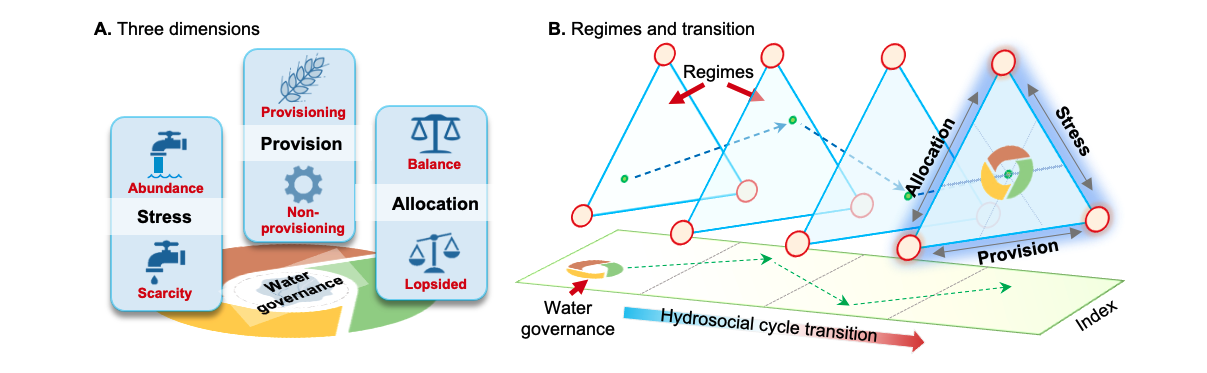
\includegraphics[width=1.1\linewidth]{main/framework.png}
	}
	\caption{
		\textbf{A.} Identifying the water governance regimes in transitions of a hydrosocial cycle with an integrated water governance index (IWGI). Water stress (S), purposes of water services (P), and water allocation (A) are three aspects to be considered.
		For example, reservoir construction (\ding{172} and \ding{173}) can relieve local water stress; The development of intensive irrigated agriculture (\ding{174}) and growth of energy industrial demand (\ding{175}) will change the purpose of water use; The water delivery system controls water allocation (\ding{176} and \ding{177}) within the basin system.
		\textbf{B.} Therefore, the methodology is to combine three aspects' corresponding indicators, and then an abrupt change of the IWGI can indicate a regime shift in water governance.
	}\label{fig:framework}
\end{figure*}


The Yellow River Basin (YRB), which contains the fifth-largest and most sediment-rich river in the world, needs integrated water governance because of geological and human history~\cite{mostern2021,best2019}.
Since the 1960s, governance practices such as reservoirs, levees, and conservation measures have contained the issues troubled by thousands of years of high sediment loads~\cite{wang2016a,song2020}.
However, new challenges such as decreased streamflows and water depletions occurred in more recent times, followed by different water governance practices like water use regulation and water transfer across basins~\cite{wang2019c}.
Today, it is still impossible to completely solve water stress, trade-offs between ecosystem services, or lopsided development in different regions in the YRB to the satisfaction of all actors~\cite{wohlfart2016}.
Governance challenges induced by environmental, economic, social, and political factors have resulted in YRB being among the most intensively-governed large river basins worldwide~\cite{nickum2021}.
Identifying regime shifts in water governance within the YRB can thus provide crucial insights into rapidly-changing big river basins and how governance may respond to meeting challenges to their sustainability.

% 这里我们整合了三个方向,提出了描绘流域人水关系的指数
Here, we depict three aspects of water governance -stress, purpose and allocation with corresponding indicators (see methods) and thus develop an Integrated Water Governance Index (IWGI) by equally weighting them, to indicate results from water governance (see Figure~\ref{fig:framework}~B).
% 使用案例研究
Then, by applying the index to a typical rapid-changing big river basin (the YRB), we show how IWGI helps detect and describe complicated water governance regimes comprehensively but straightforwardly.
Following synthetic analyses of the changes in water demand, supply, economic outcomes, and institutions, we interpret the leading causes of the regime shifts.
% 最后总结出一般性框架
Finally, we propose a general regime transition schema that offers a practical guideline for a coordinated approach to exploring the challenges faced by big river basin governance.


% Headings should be sentence fragments and do not begin with a
% lowercase letter or number. Examples of good headings are:
\section{Materials and Methods}\label{sec11}
The aim of this analysis was to develop a transparent and easily replicable approach to identifying water governance regimes and regime shifts; thus, it is not intended to provide a comprehensive model of social-ecological water dynamics. We constructed the Integrated Water Governance Index (IWGI) based on three dimensions (supply, purpose, allocation, see Figure 1) selected a priori and identified the changes in periods of the index over time using change point detection. Each dimension is reflected by an independent indicator after normalization, and water governance regimes were characterized by the combination of impacts along each dimension at different time periods. The contribution to changes of IWGI index along with each main indicator were also decomposed and calculated separately for each regime period.

\subsection{Integrated Water Governance Index (IWGI)}

Our Integrated Water Governance Index offers an accessible and operational way of measuring regime changes based on the transparent underlying assumptions that water resources governance system is closely related to a transformation towards a hydrosocial water cycle in the three dimensions below (see Figure 1 and SI 322 Appendix Methods S4 for details)
\cite{abbottwatercycleAnthropocene2019,leviaHomogenizationterrestrialwater2020,steffenTrajectoriesEarthSystem2018}.

	% - 社会的发展通常伴随着用水向社会经济系统倾斜,用水方式优先向收益更高的非供给性方式倾斜:
	\begin{itemize}
		% - 可持续的社会发展应该通过技术手段有效缓解发展过程中产生的水资源压力,才能实现可持续发展:
		\item \textbf{Supply($S$)}: Socio-economic dominance may lead to further demands on the water supply because of increasing water withdrawals. However, since effective water governance may boost supply capacities to meet water demands by technical solutions in the process of development:
		\begin{equation}
			Transformation \propto S^{-1}
		\end{equation}


		\item \textbf{Priority($P$)}: Transformation is usually accompanied by a change of purpose in water governance towards socio-economic services (usually towards non-provisioning purposes), because of higher returns:
		\begin{equation}
			Transformation \propto P
		\end{equation}

		% - 社会发展通常伴随着更具结构性的水资源配置,如区域部门之间的分工合作,以及区域的统筹配置:
		\item \textbf{Allocation($A$)}: Transformation usually leads to more complicated structures in water allocation, as a result of division and cooperation between regions and sectors because of environmental context and economic comparative advantages:
		\begin{equation}
			Transformation \propto A
		\end{equation}

	\end{itemize}

	% 将三者合一起,即:
	We combined these three dimensions into a single integrated index, keeping their positive or negative relationship with the transformation towards a hydrosocial water cycle:
	\begin{equation}
		Transformation \propto P*A*S^{-1}
	\end{equation}

	% 在上述假设的基础上,我们要构建流域综合耦合指数(Integrated Water Resources governance, IWGI),使 IWGI 有效表征与用水相关的三个维度。首先为每个维度选择一个合适的指示因子(indicator, $I_x$, 其中$x=P, C or S$)。将上式进行自然对数转换,从而让三个维度之间变成加减关系:
	To effectively represent the three dimensions, we selected an appropriate indicator ($I_x$, $x=S$, $P$ or $A$ corresponding to supply, purpose, and allocation respectively) for each dimension. Then, the above equation was transformed into a natural logarithm to facilitate calculation:
	\begin{equation}
		Transformation \propto ln(I_S) + ln(I_P) - ln(I_A)
	\end{equation}

	Assuming they have equal weights, the Integrated Water Governance Index (IWGI) is:
	\begin{equation}
		IWGI = I'_S + I'_P - I'_A
	\end{equation}

	where $I'_x$ is a normalization of log-transformed indicator $I_x$ for a certain dimension:
	\begin{equation}
		I'_x = normalize(ln(I_x))
	\end{equation}

	\subsubsection*{Normalization}
	We tested different normalization methods, and they made no difference in change points detection (see \textit{SI Appendix} Methods S5. Sensitivity analysis). We performed min-max normalization using the formulation below:
	\begin{equation}
		normalize(X) = (X - X_{min}) / (X_{max} - X_{min})
	\end{equation}

	\subsubsection*{Indicator of supply}
	We used the scarcity-flexibility-variability (SFV) water stress index proposed in Qin et al., 2019 to evaluate water supply capacities ($SFV_i$) as the indicator in a certain region $i$ \cite{qinFlexibilityintensityglobal2019}. This metric takes into account management measures (such as the construction of reservoirs) and the impact of changes in the industrial structure of water use on the evaluation of water scarcity (see \textit{SI Appendix} Methods S4 for details). For the whole YRB, the indicator of supply capacity $I_S$ is the average of all regions' SFV-index:
	\begin{equation}
		I_S = \frac{1}{4} * \sum_{i=1}^4 SFV_{i}
	\end{equation}

	Where $SFV_i$ is the SFV-index for region $i$, and $i=1$ to $4$ refers SR, UR, MR, and DR (see \textit{SI Appendix} Methods S1 Definition of study area).

	\subsubsection*{Indicator of purpose}
	To quantify purpose $I_P$, we used Non-Provisioning purpose Shares (NPS) of water use as an indicator. While provisioning purpose water use ($WU_{pro}$) includes domestic, irrigated and livestock water uses, non-provisioning purpose water use ($WU_{non-pro}$) includes industrial and urban services water uses. We calculated the NPS as:
	\begin{equation}
		NPS_{i} = \frac{WU_{non-pro, i}}{WU_{pro, i} + WU_{non-pro, i}}
	\end{equation}

	Where $i$ refers a certain region, or the whole basin, i.e:
	\begin{equation}
		I_P = NPS_{basin}
	\end{equation}

	\subsubsection*{Indicator of allocations}
	%$AEM$ 指标度量的是水资源配置“不均匀”的程度,类似于信息熵是对“混乱程度”的度量,即参与分配的各个单位之间,分配比例差距越大,则熵越小。
	% 而我们的指标应反映随着社会发展,水资源配置在区域之间更加均衡(比例差距小)、整体满足不同用水部门的发展需求(比例差距减小)、但不同区域存在部门分工(比例差距增大)的趋势。
	To describe allocations $I_C$, we designed an indicator based on information entropy, called Allocation Entropy Metric (AEM), AEM measures the degree of evenness of water allocation (see \textit{SI Appendix} Methods S4).
	Our indicator $I_C$ was intended to reflect the idea that with the development of society, water resources allocation becomes more balanced among regions and generally meets the needs of different sectors, but different regions have a trend of division of labour among various sectors (with larger gaps):
	\begin{equation}
		I_C = \frac{AEM_{r}*AEM_{s}}{AEM_{rs}}
	\end{equation}

	where $AEM_{r}$ and $AEM_{s}$ are Allocation Entropy Metric in different regions and different sectors. $AEM_{rs}$ describes differences between sectors in a certain region relative to the whole basin (see \textit{SI Appendix} Methods S4).

	\subsection{Change points detection}
		% The method makes no assumptions about the distribution of the data and detects breakpoints based solely on the probability of the data coming from different distributions before and after the breakpoint.

		With no assumptions about the distribution of the data, the Pettitt (1979) approach of change-point detection is commonly applied to detect a single change-point in hydrological time series with continuous data
        \cite{pettittNonParametricApproachChangePoint1979}.
		It tests $H0$: The variables follow one or more distributions that have the same location parameter (no change), against the alternative: a change point exists. The non-parametric statistic is defined as:
		\begin{equation}
			K_t = max|U_{t, T}|
		\end{equation}

		Where:
		\begin{equation}
			U_{t, T} = \sum_{i=1}^t\sum_{j=t+1}^T sgn(X_i - X_j)
		\end{equation}

		The change-point of the series is located at $K_T$, provided that the statistic is significant. We used 0.001 as the threshold p-value (see \textit{SI Appendix} Methods S5 for Sensitivity analysis), meaning that the probability of a statistically significant change-point judgment being valid was more than $99.9\%$.
		Since this method can only return one significant change point, we repeated it until all significant change points were detected.

	% 计算贡献度
	\subsection{Contribution decomposition}
		We decomposed the amount of variation in each index at different periods to quantify each influence's contribution to the index. Using the Integrated Water Resources governance (IWGI) Index as an example, its value is influenced by normalized indicators in three dimensions: stress ($I'_S$), purpose ($I'_P$) and allocation ($I'_C$). We can calculate their differences between two certain years ($y_2$ and $y_1$, $y_2 > y_1$) by:
		\begin{align}
		\Delta IWGI &= (I'_{P_{y_2}} + I'_{C_{y_2}} - I'_{S_{y_2}}) - (I'_{P_{y_1}} + I'_{C_{y_1}} - I'_{S_{y_1}}) \\
		&= (I'_{P_{y_2}} - I'_{P_{y_1}}) + (I'_{C_{y_2}} - I'_{C_{y_1}}) + (I'_{S_{y_1}} - I'_{S_{y_2}}) \\
		&= \Delta I'_P + \Delta I'_C + (-\Delta I'_S)
		\end{align}
		Then, the contribution of dimension $x$ to IWGI's changes can be referred to as:
		\begin{equation}
			Contribution_x = \frac{\Delta I'_x}{\lvert \Delta IWGI \rvert}
		\end{equation}

		% Since $Contribution_x$ can be positive or negative, we used an absolute value to evaluate the contribution (in proportion) of a certain dimension in the all three dimensions to the changes:
		% $$  Contribution_x\% = \frac{|\Delta I'_x|}{\sum_x |\Delta I'_x|} $$

		% or just for contributions (in proportion) within a certain year $j$ to the regime:
		% $$ Contribution_{x,j}\% = \frac{|I'_{x, j}|}{|\sum_x I'_{x, j}|} $$

	\subsection{Datasets}
	% 为了计算 IWGI ,我们需要计算多个指标及子指标,所有使用的数据集都在表中列出,数据的详细介绍可见补充材料。
	In order to calculate IWGI, we need to calculate multiple indicators and sub-indicators. All the datasets used are listed in the \textit{SI Appendix} table S1. A detailed description of the data is provided in the supplementary materials \textit{SI Appendix} Methods S2.

% \section{Materials and Methods}
% Here is text on Materials and Methods.
%
% \subsection{A descriptive heading about methods}
% More about Methods.
%
% \section{Data} (Or section title might be a descriptive heading about data)
%
% \section{Results} (Or section title might be a descriptive heading about the
% results)
\section{Results}\label{sec2}
\subsection{Water governance regimes}
\label{Res.1}

\begin{figure*}[ht!]
	\centering
	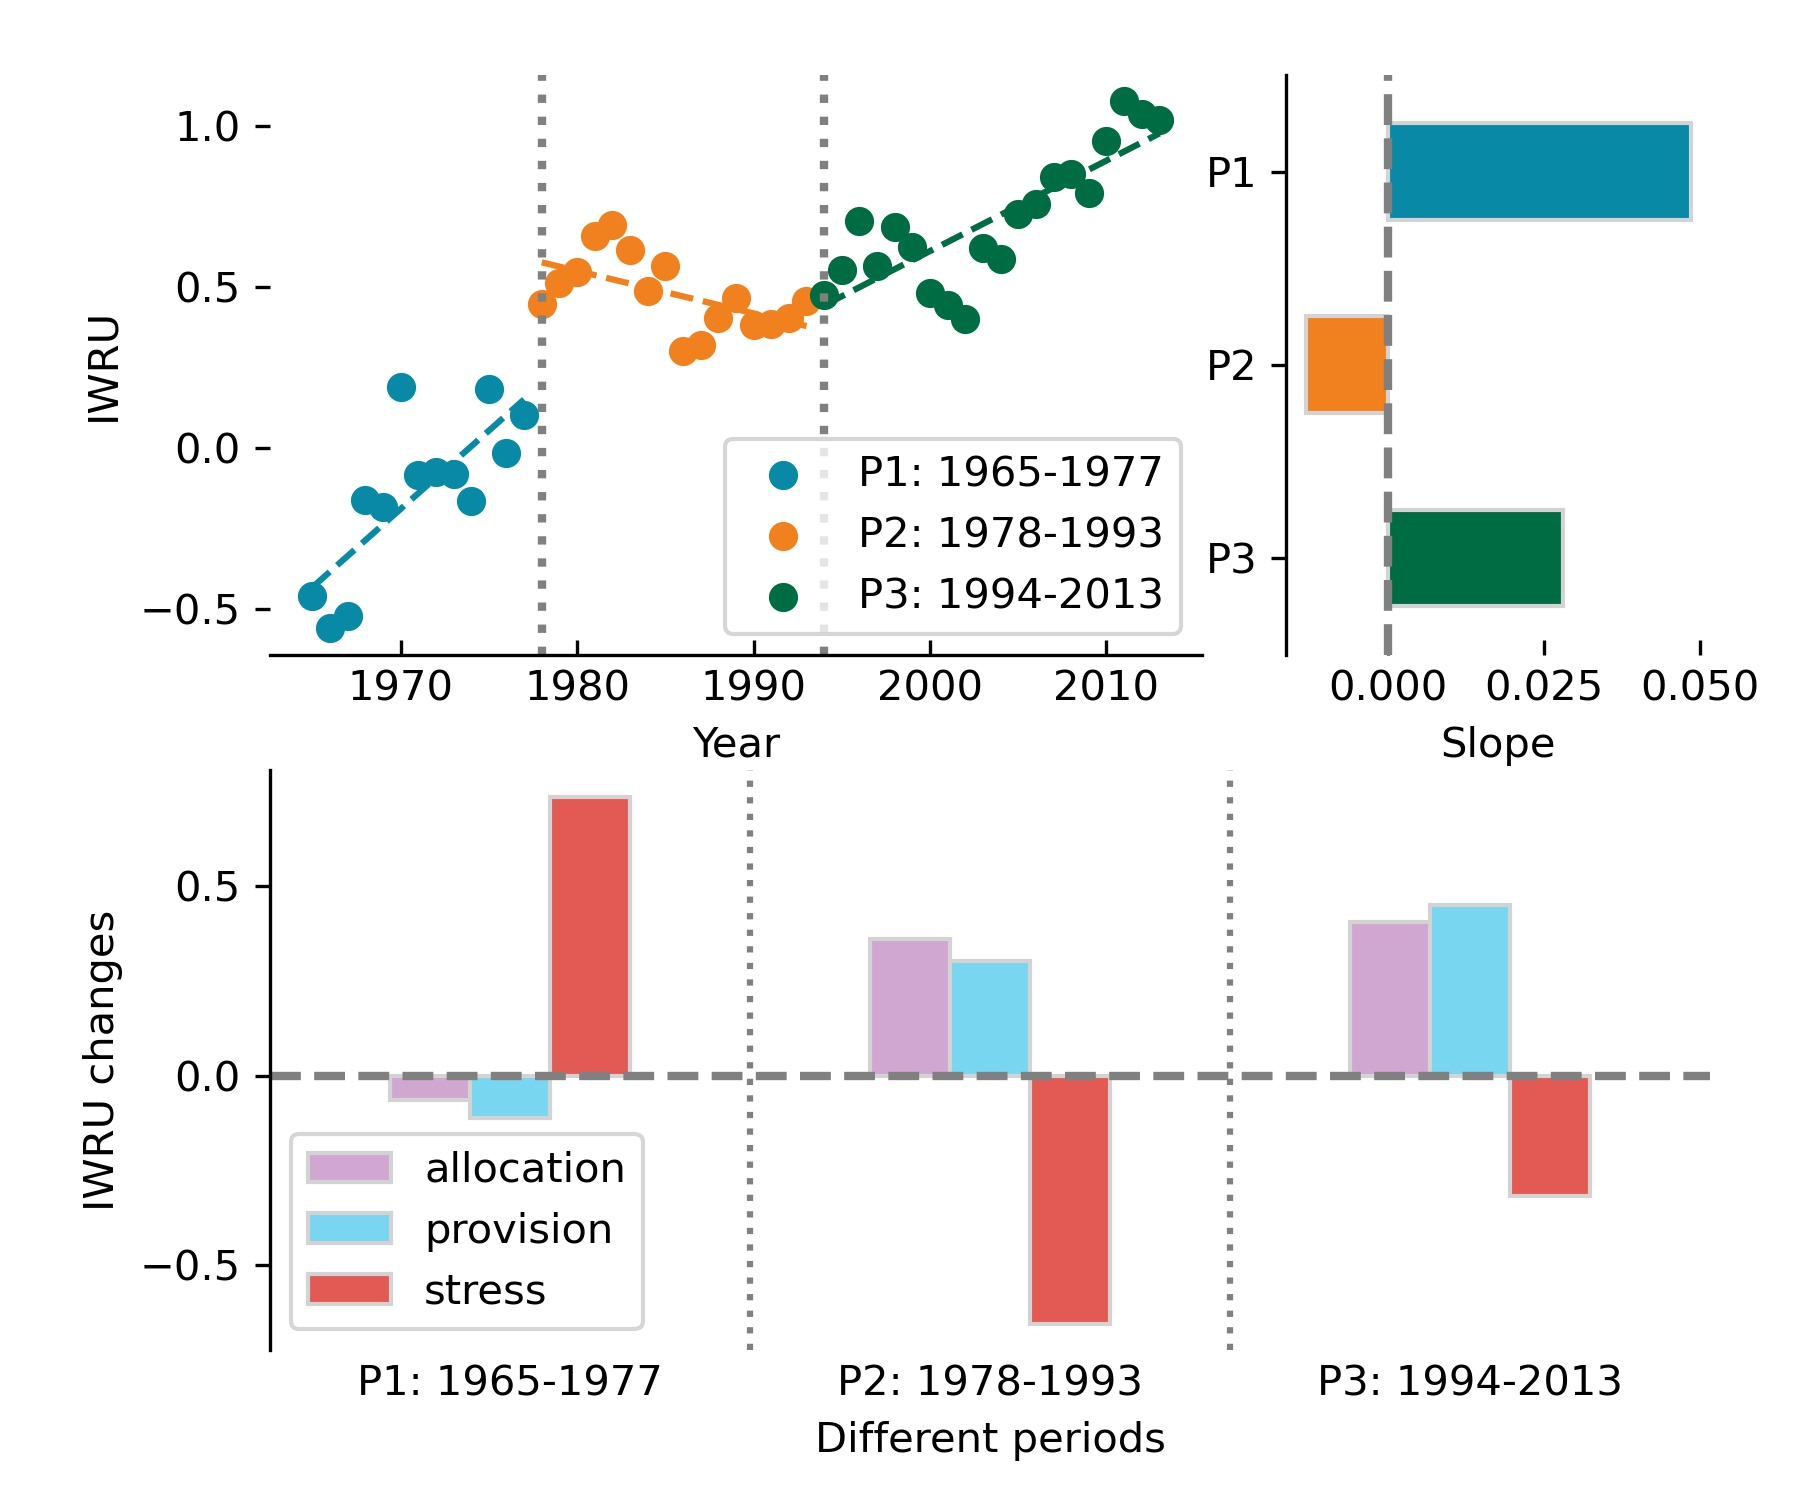
\includegraphics[width=0.9\linewidth]{main/index.jpg}
	\caption{Changes in the IWGI index and corresponding water governance regimes: P1: 1965-1978, P2: 1979-2001, and P3: 2002-2013.
	\textbf{A,} detecting change points of IWGI and contributions from each indicator. Two significant change points ($p<0.01$) occurred in 1978 and 2001.
	\textbf{B,} correlation of trends between the IWGI and the indicators.
	\textbf{C,} across three indicators, changing components of the IWGI, whose directions shifts between different regimes.
	}
	\label{fig:IWGI}
\end{figure*}

% 这一节主要展示IWGI的变化趋势和WUR的划分
Two significant breakpoints divide the changes in the IWGI into three periods, with different contributions from three aspects (Figure~\ref{fig:IWGI}A).
% 第一阶段
In the first period (P1, 1965-1978), the IWGI decreased rapidly.
While the indicator of purpose and allocation contributed more to the IWGI ($49.45\%$ and $34.95\%$ on average, respectively), the remarkable downward trend correlates significantly ($p<0.01$) to the decreasing allocation and stress indicators (Figure~\ref{fig:IWGI}B).
% 第二阶段
In the second period (P2, 1979-2001), the increasing stress indicator significantly ($p<0.01$) contributed to the upward IWGI, while the allocation and purpose indicators played negative roles in changing the IWGI.
% 第三阶段
During the third period (P3, 1995-2013), while the stress indicator kept its most prominent share in contributions ($57.11\%$ on average), the increased allocation indicator and decreased purpose indicator changed the regime.
% Overall
Taken together, the overall features of the three aspects in different periods are relative to a directional change in the combination of three aspects (Figure~\ref{fig:IWGI}C).

\subsection{Causes of the regime shifts}
\label{Res.2}

\begin{figure*}[th!]
	\centering
	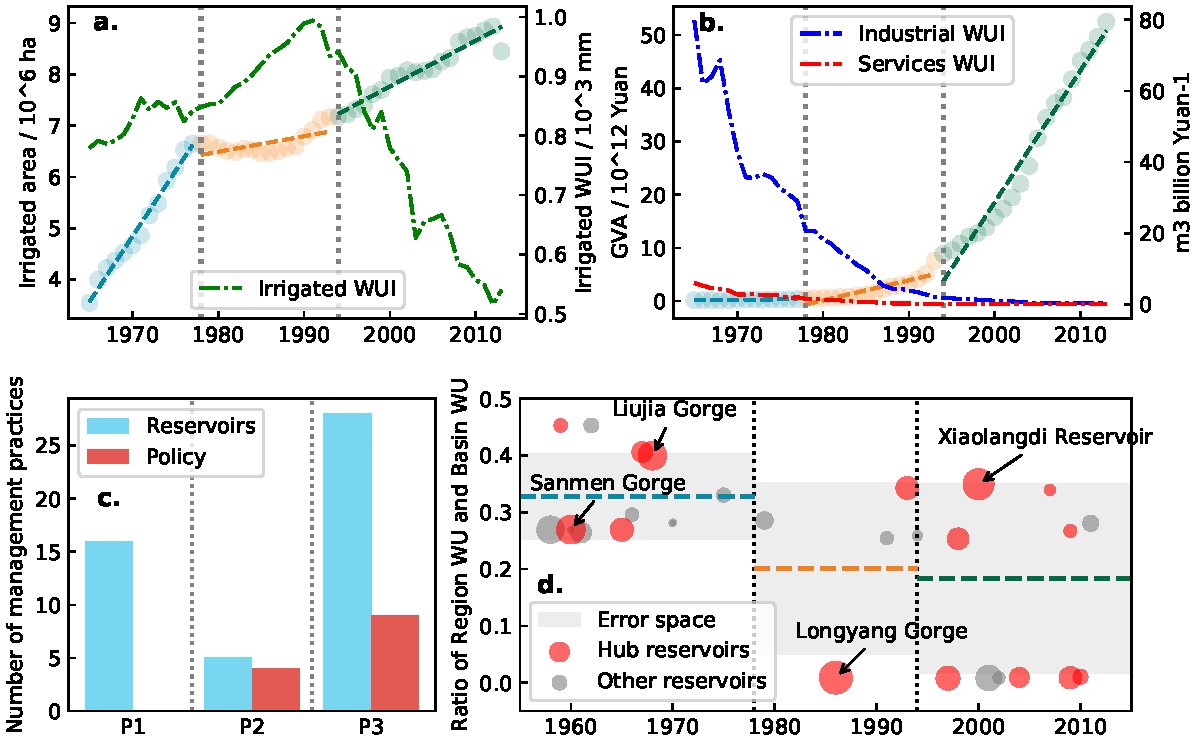
\includegraphics[width=0.9\linewidth]{main/causes.pdf}
	\caption{
		Causes of water governance regime shifts in the YRB.
		\textbf{A.} Changes in the total irrigated area (orange line) and water use intensity ($WU/A$, water use divided by the irrigated area, the green dot line).
		\textbf{B.} Changes in gross values added (GVA) of industry and services (blue line) and their water use intensities ($WU/GVA$ WU divided by the GVA, the red dot line).
		\textbf{C.} Completed time of each new reservoir and their located region's water use (LWU) percentages as a proportion of the total basinal water use (BWU) at that time. Red circles denote the reservoirs mainly for managing and regulating the whole basin.
		The size of each circle indicates the magnitude of its water storage capacity.
		\textbf{D.} Social transformations (red triangles) and national-level governance policies (the circles, different colours denote signed by different state institutions, see \textit{Appendix} Table~\ref{tab:policies}). The light grey bars count official documents related to the YRB on a basinal scale (the Yellow River Events).
	}
	\label{fig:Causes}
\end{figure*}

% 进一步挖掘IWGI变化的根本原因,
The underlying causes of changes in the IWGI are different in the two regime shifts.
% 灌溉区扩张和工业和服务业的经济增长是P1和P2目的变化的关键。
Changing water demands and supply were critical to the shift between P1 and P2.
% P1年,黄河流域灌溉农业面积以图A的速度快速扩张,灌溉用水占主导(1965年占总用水的$81.56\%$, 1978年占总用水的$83.17\%$,图S3)。
As the dominant water demand during the P1, the area of irrigated agriculture in the YRB expanded rapidly at a rate of $0.25*10^6 ha/yr$ (Figure\ref{fig:Causes}~A), simultaneously supported by increasing supply through the construction of reservoirs (\textit{Appendix} Figure~\ref{fig:reservoirs}).
% 然而,进入P2后,灌溉区扩张停滞,工业和服务业逐渐增长,用水需求增加(图re\ref{fig: Causes} B),导致灌溉用水量比例下降$8\%$ S3。
Ensuing the P2, however, the expansion of irrigated areas slowed down, and industry and services gradually took off (Figure\ref{fig:Causes}~A and B).
% 水分利用效率由P2变化到P3。
Then, the efficiency of water use changed obviously from P2 to P3.
Not only did irrigated areas continue to expand slowly during the P3 (Figure\ref{fig:Causes}~A), but industry and urban services also assumed a more vital economic role (represented by Gross Added Values, GVA) (Figure~\ref{fig:Causes}~B).
Because of increased efficiency, however, they both experienced significant declines in water use for a unit irrigated area or unit production (Figure~\ref{fig:Causes}~A and Figure~\ref{fig:Causes}~B).
As a result, the differences between sectors and regions in water use reduced while the total water stress steadily remained high during the P3 (Figure~\ref{fig:IWGI}A).

% 最后,环境背景、社会转型和水治理政策在这三个时期都发挥了作用。
Environmental context, social transformation, and policies played roles in all three periods.
We calculated the ratios of regional and basinal water use for each reservoir (R/B ratio) (Figure~\ref{fig:Causes}C), with a higher ratio representing a potential role in water supply rather than basinal regulations.
Under the banner of ``conquering nature'' most of the reservoirs were built in regions with high water demands during the P1 (R/B ratios were significantly higher ($p<0.01$, see Figure~\ref{fig:Causes}C)).
Ensuing the P2, the number of new reservoirs decreased significantly and significantly increased basin policies rigorously controlled the allocation of water (Figure~\ref{fig:Causes}D, $p<0.01$ and \textit{SI Appendix} Figure~\ref{fig:reservoirs}).
During the P3, authorities proposed more national-level water governance policies under the guidance of the national strategy ``environmental regulation'' (Figure~\ref{fig:Causes}D).
The regime shift from P1 to P2 is in line with the increasing water supply and demands; while driven by regulatory policies and efficiency enhancement under stable water stress from P2 to P3.


% \section{Conclusions}

\section{Discussion}\label{sec12}

% Implications
Water governance gradually becomes a national or international concern from a primarily local concern because large river basins are critical sources of ecosystem services, economic development, and human well-being~\cite{best2019,best2020}.
As tele-coupling raises additional water governance challenges in an increasingly tightly-connected world, regime shifts in water governance align with different human-water relationships~\cite{diaz2019}.
The process echoes how societies have been proposed to change governance practices by enhancing their adaptive capacity in the hydrosocial cycle~\cite{loch2020,turton1999}, and the IWGI quantitatively identifies this transition.
It is vital for scientists and decision-makers to recognize the changing governance challenges because models, institutions, engineering, and approaches developed under one regime are not necessarily applicable under a different regime~\cite{reyers2018}.

% 我们为的研究结果表明,黄河流域能被识别为三个明显的稳态。
In the case of the YRB, our results show that there have been three distinct governance regimes; we named them: a massive supply regime (P1: $1965 \sim 1978$), a governance transforming regime (P2: $1979 \sim 2001$), and an adaptation oriented regime (P3: $2002 \sim 2013$) (Figure~\ref{fig:IWGI}).
During the massive supply regime with lower water stress ($1965 \sim 1978$ in the YRB), water governance thus tended to boost water supply for services (mainly provisioning purposes then -livestock and crops) by constructing reservoirs and channels (Figure~\ref{fig:Causes}~B).
As the Chinese slogan ``human will conquer nature'' suggested then, however, the enhancement of water supply did not align with irreversible changes in the human-water relationship; it drastically increased water demand with little consideration for ecological conservation~\cite{zhou2020}.
The rapid expansion of irrigated farmland and water diversion facilities in the same decade brought the overburdened YRB close to a critical point (Figure~\ref{fig:Causes}), where increasing supply to meet demand was impractical~\cite{loch2020}.
Use of over $80\%$ of the surface water since 1972 has led to frequent river depletion, causing additional ecological issues such as wetland shrinkage and declines in biodiversity~\cite{wang2019c}.
In addition, since water stress also limited the growing industrial economy, the existing modes of water governance led to a social-ecological crisis~\cite{wohlfart2016}.

The start of the governance transforming regime (P2: $1979 \sim 2001$) coincided with rising competition for water use after the ``reform and opening-up'' (Figure~\ref{fig:Causes}~C).
% 正如理论预测的那样
The results from the YRB mirror those of the theoretical analysis: continuous increases in water demand when the basin's total supply is stable can follow substantial changes in governance regime and a rapid enhancement in overall social adaptive capacity~\cite{loch2020}.
% 作为制度转变的先行者
As a pioneer in shifting governing institutions, the YRB triggered institutional changes during this regime. These include, for example, slowing the growth of irrigated acreage and leading water-saving infrastructure (Figure~\ref{fig:Causes}); creation of China's first water quota scheme, and the creation of a preliminary cross-boundary water transfer plan~\cite{wang2019e,long2020,nickum2021}.
% 因此,1999年黄河的最后一次枯竭
Consequently, although water stress remained and increased (due to reducing streamflow and flexibility), the last depletion of the Yellow River in 1999 led to a climax in this transformation in water governance~\cite{wang2019e}.

The ensuing adaptation-oriented regime (P3: $2002 \sim 2013$) involved a significant societal shift in adapting to stable high water stress.
% 一个基本背景是,在用水量总体保持稳定的情况下,黄河流域的径流量已显著低于从前,这是该时期水资源压力重新上升的重要原因。
Partially because of changed climate~\cite{han2023,liu2020c}, the runoff of the YRB was significantly lower than before when the overall water uses remained stable, which was an important reason for the rise of water stress in this stage (Supplementary Materials Figure~\ref{fig:runoff} and Figure~\ref{fig:scarcity}).
Socio-economic trade-offs between water-dependent regions and sectors, however, played a more important role in this regime, so water governance had to achieve efficient water allocation while balancing different demands in the face of limited water supply~\cite{dalin2015,song2022}.
Widespread reconstruction of resources in different industries and regions led to calls for adaptation in water governance, using the urgent requirements of adjusting rigid quota shares from the previous regime as an example~\cite{wang2019e}.
Many national-level governance practices were proposed under the regime because the absence of such policies to support high-quality development became new a structural challenge for water governance~\cite{konar2019}.

% 总体而言,长江流域的水治理是“改善供给、转变治理、增强适应”的水社会循环总体转型中最突出的例子之一。
In general, water governance of the YRB is among the most prominent example in the widespread transition to a hydrosocial cycle -``improving supply, transforming governance, and enhancing adaptation''.
To support water use in early stage (Figure~\ref{fig:summary}~A), strategies tend to manage natural water processes in order to maintain the provisioning (larger) and non-provisioning water (less).
At the later stage (Figure~\ref{fig:summary}~B), emphasis is governing across the whole basin, water governance practices are adaptively designed to meet the increasing needs of the socio-economic system and carried out.
With the above gradually shifting, the emergence of different regimes drives water governance challenges at a basin-scale: these were primarily economic and environmental before the transformation, but social and policy-related towards the end (Figure~\ref{fig:summary})~\cite{singh2019,porcher2019}.
In an analogy at a global scale, the resource challenges, represented by water shortage and water supplying difficulties, are mainly faced by undeveloped and developing basins~\cite{allan2019,speed2013,liu2012}.
Highly-controlled and developed basins (especially for transboundary rivers) must mainly resolve structural challenges, such as water disputes or lack of equity, and may be in urgent need of novel flexible, efficient sociopolitical governance structures~\cite{unep-dhi2016,mirumachi2015}.
Linking regime shifts to the governance challenges, the implementation of IWGI thus offers a comprehensive and straightforward way to interpret the intertwines between water governance and the hydrosocial transition.

Future's tightly intertwined socio-hydro interactions can lead water governance challenges even more complex and comprehensive, combining resources issues and structural barriers~\cite{huggins2022a}.
For example, climate change may alter water scarcity levels and make it more difficult to effectively use water due to extreme climate events, strengthening water stress and threatening infrastructures~\cite{liu2017, dibaldassarre2019}.
Additionally, adapting to climate change could lead to transformations~\cite{sachs2019,barnes2020}, prompting a reevaluation of governance strategies of social water usage (priority and allocation) which is being increasingly altered by current regime transitions.
It may be difficult to exhaust what is considered in a good watershed governance strategy, but the IWGI at least gives us a sense of where the a river basin is heading and how challenged.

\begin{figure*}[htbp!]
	\centering
	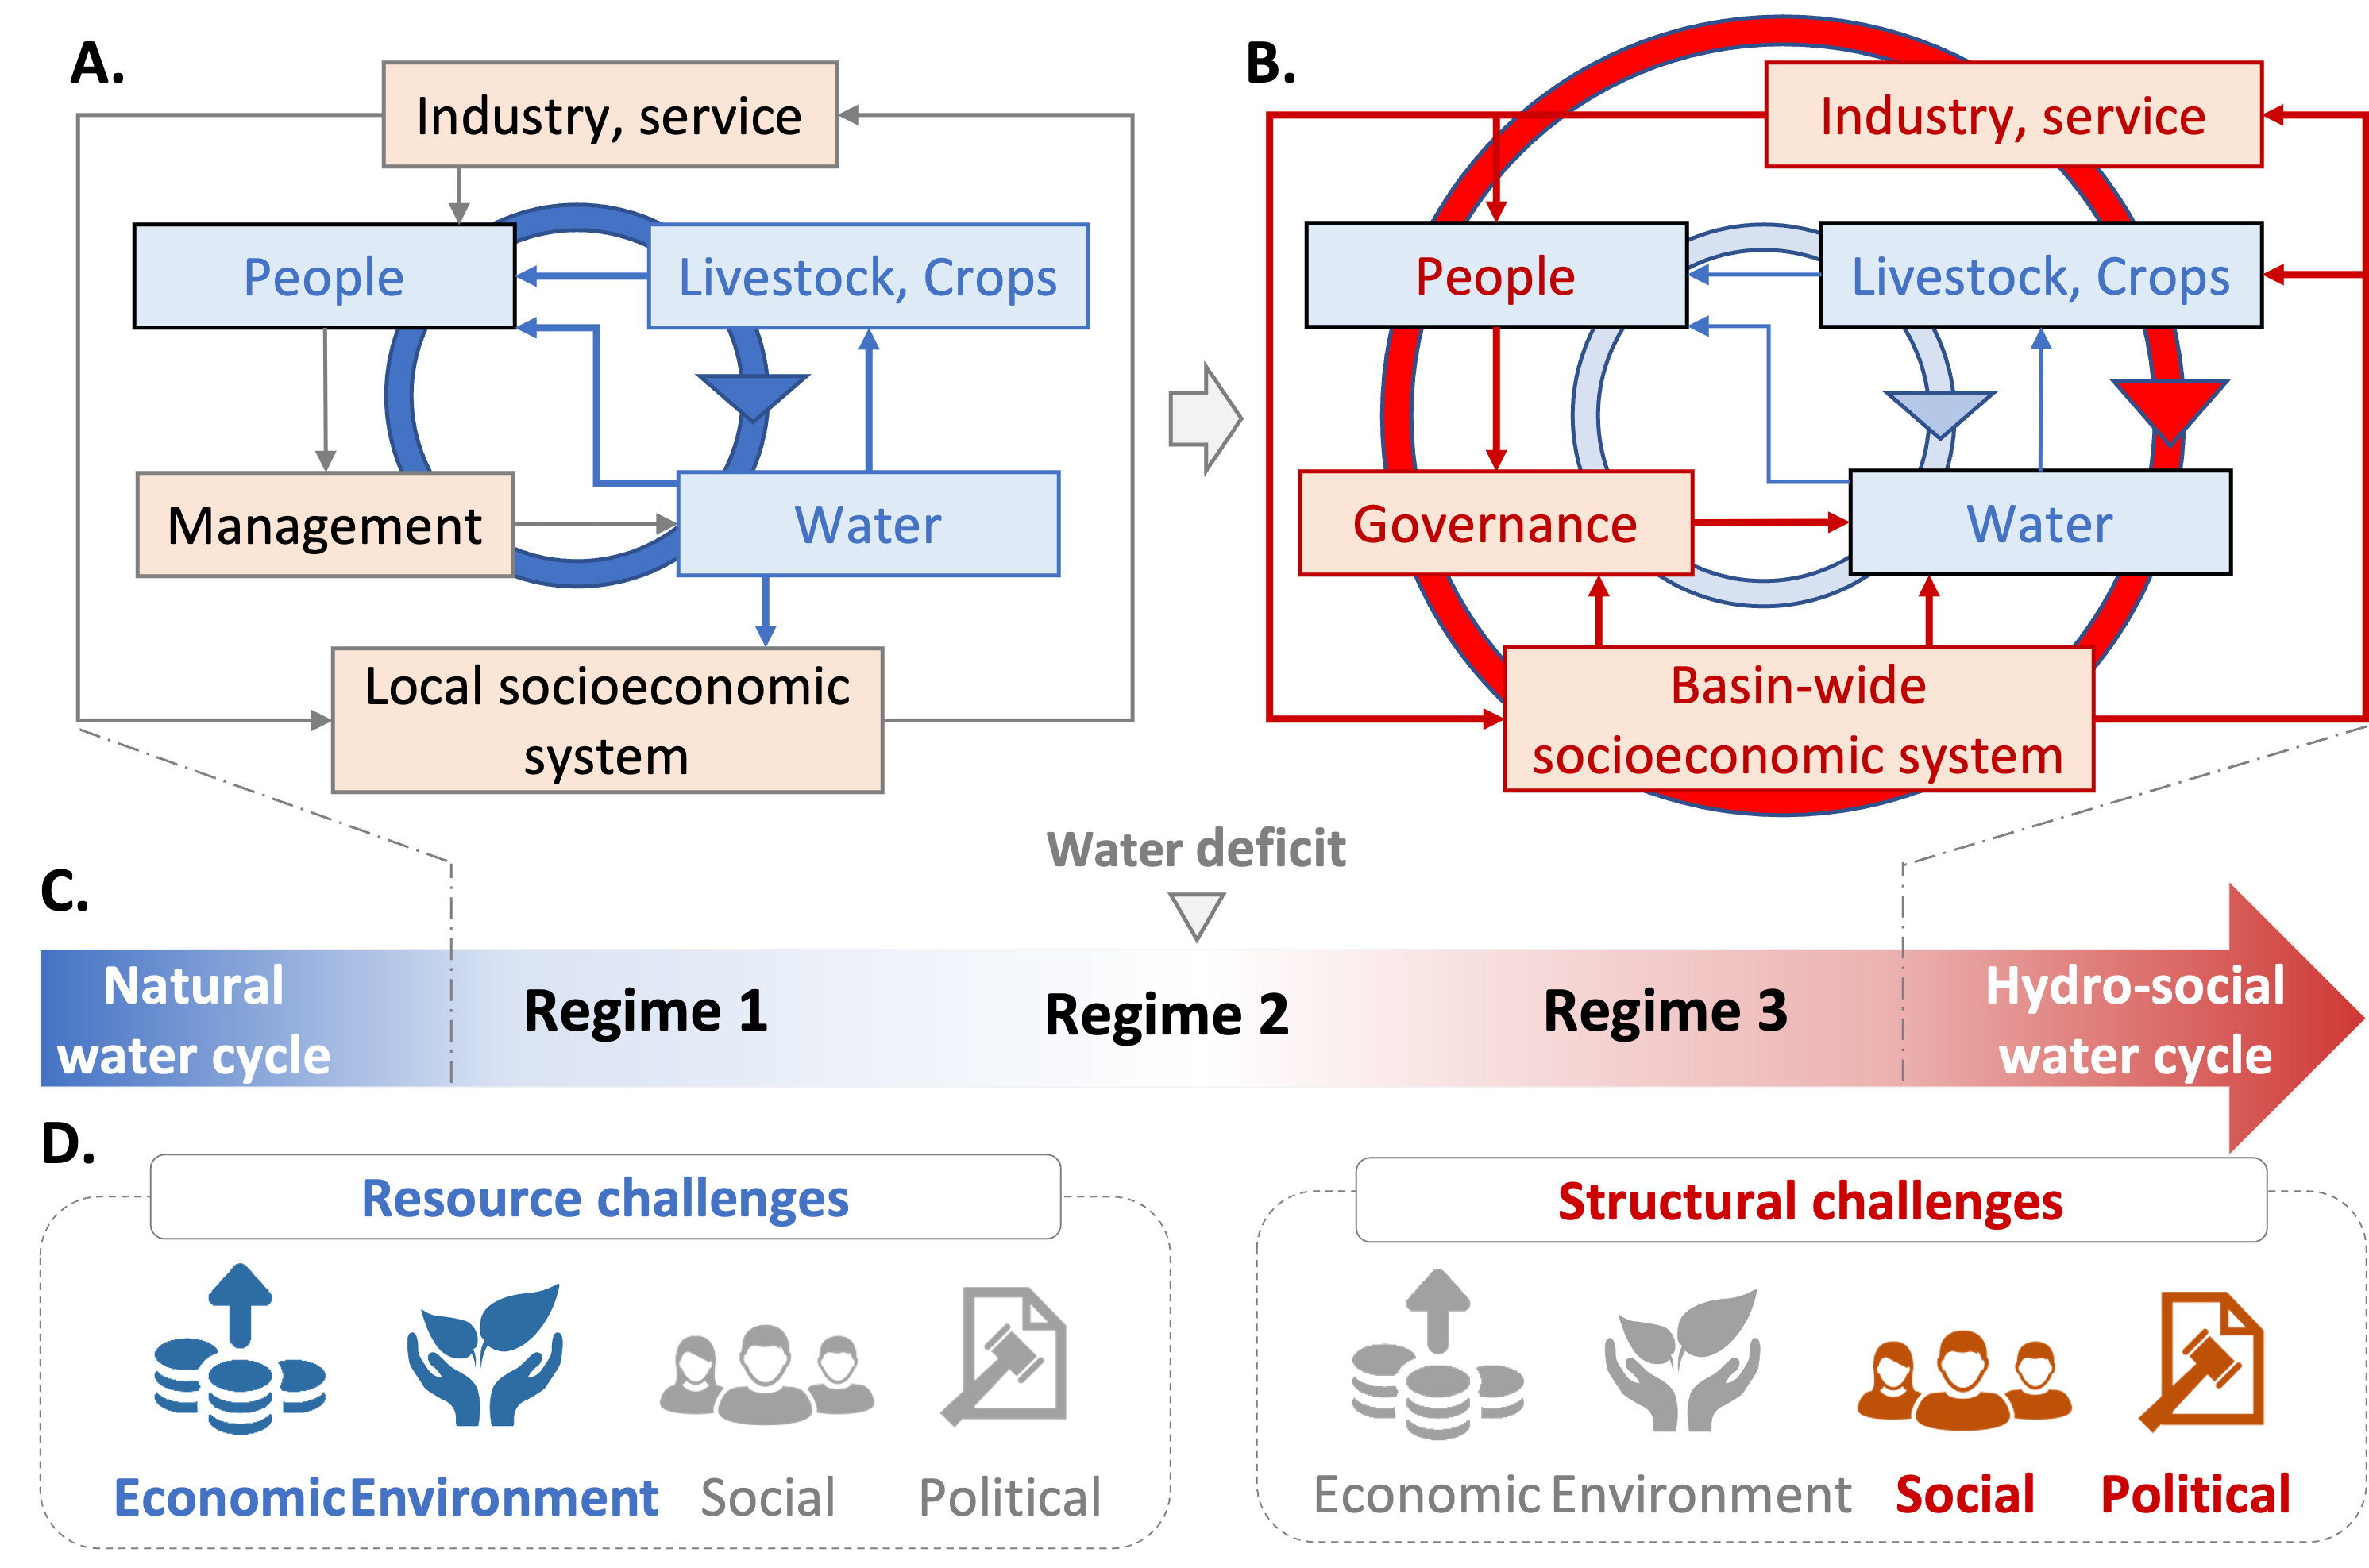
\includegraphics[width=0.8\linewidth]{main/transition.png}
	\caption{
		Transition schema in hydrosocial cycle and water governance regimes. The natural water cycle dominates blue pathways, while socio-economic feedback dominates red.
		The large circular arrows indicate the social and hydrological processes that dominate in different stages.
		Provisioning water includes water used by human, livestock and crops while non-provisioning water includes used by industry and service.
		The processes expressed in the graph mainly include: Water supports people in provisioning ways or influence/influenced socioeconomic systems as non-provisioning ways; People manage/govern water system based on their well-beings.
		The gray thick arrow represents weaker process, while the red arrow represents more significant one.
		\textbf{A.} As socio-economic systems develop, non-provisioning water demand increases; simultaneously, increased adaptive capacity by engineering allows people to manage water resources to alleviate water stress.
		\textbf{B.} With further growing socio-economic systems, trade-offs between provisioning-purpose and non-provisioning water use become prominent; a basin-wide socio-economic system requires more organized water governance.
		Thus, \textbf{C. the hydrosocial water cycle transition} correlates with the water governance regime shifts. The transformation governance regime shift occurs following the water deficit, with the rapid growth of adaptive capacity.
		\textbf{D. Water governance challenges} Through the transitional regimes, water governance faces primarily economic and environmental challenges but social and policy challenges later.
	}\label{fig:summary}
\end{figure*}


%* limitations & direction
One of the main limitations in the approach is the lack of multi-sources data in long-term period worldwide, which means there is still a gap between comprehensively identifying and applying the IWGI widely.
We propose that all water governance issues, however, can change ``who gets water, when and how'' so monitoring such an integrated index is essential, even use simpler indicators.
We suggest that choices of indicators for different aspects can be adopted according to available datasets -e.g., replace the SFV-index (IA) with simpler scarcity index or proportion-based priority indicator (IP) by complicated one.
Another limitation is the lack of latest datasets which is coherent with the historical datasets, so our analysis had to discontinued in 2013 despite potential shifts existing.
As a supplement, we examined IWGI framework with fewer datasets from different source in recent decades where showing no significant regime changes (supplementary Figure~\ref{fig:summary}).  % TODO 补充材料新图
Therefore, we suggest IWGI framework can be applied with adaptive indicators and flexible time series according to accessible datasets in future studies.

In today's world, regime shifts from natural to human-dominated seem likely to become increasingly widespread; comprehensive strategies to address governance challenges will have to become the core of complex human-water systems~\cite{cumming2018,cumming2014,jaeger2019}.
Although river basins have shown improvements in water management technologies and water use efficiency, many are still approaching local, regional, and planetary boundaries where human-water systems may collapse~\cite{gleeson2020, wang-erlandsson2022}.
A deeper understanding of governance that incorporates ideas of non-linear regime shifts and transformations should help shift the focus of governance towards maintaining the resilience of the basin’s social-ecological system and improving its sustainability~\cite{falkenmark2019}.


\section{Conclusion}\label{sec13}

Three dimensions of water governance change along with the hydrosocial cycle transition: water stress, services purpose, and water allocation, affecting ``who gets water, when and how''. We developed an Integrated Water Governance Index (IWGI) to detect regime shifts in water governance by integrating them. Applying the index to a rapidly-changing large river basin (the Yellow River Basin, China) describes how water governance shifts between three regimes over half a century (massive supply regime; governance transformation regime; and adaptation oriented regime, respectively). Our approach quantitatively identifies the general schema for water governance regimes in the YRB, in line with previous theoretical analysis with a representative transition process. Linking regime shifts to the underlying causes, the implementation of IWGI offers a comprehensive and straightforward way to interpret changes in intertwines of water governance, hydrosocial transition, and human-water relationships.



% \section{= enter section title =}
%Text here ===>>>


%%

%  Numbered lines in equations:
%  To add line numbers to lines in equations,
%  \begin{linenomath*}
%  \begin{equation}
%  \end{equation}
%  \end{linenomath*}



%% Enter Figures and Tables near as possible to where they are first mentioned:
%
% DO NOT USE \psfrag or \subfigure commands.
%
% Figure captions go below the figure.
% Acronyms used in figure captions will be spelled out in the final, published version.

% Table titles go above tables;  other caption information
%  should be placed in last line of the table, using
% \multicolumn2l{$^a$ This is a table note.}
% NOTE that there is no difference between table caption and table heading in the final, published version
%
%----------------
% EXAMPLE FIGURES
%
% \begin{figure}
% \includegraphics{example.png}
% \caption{caption}
% \end{figure}
%
% Giving latex a width will help it to scale the figure properly. A simple trick is to use \textwidth. Try this if large figures run off the side of the page.
% \begin{figure}
% \noindent\includegraphics[width=\textwidth]{anothersample.png}
%\caption{caption}
%\label{pngfiguresample}
%\end{figure}
%
%
% If you get an error about an unknown bounding box, try specifying the width and height of the figure with the natwidth and natheight options. This is common when trying to add a PDF figure without pdflatex.
% \begin{figure}
% \noindent\includegraphics[natwidth=800px,natheight=600px]{samplefigure.pdf}
%\caption{caption}
%\label{pdffiguresample}
%\end{figure}
%
%
% PDFLatex does not seem to be able to process EPS figures. You may want to try the epstopdf package.
%

%
% ---------------
% EXAMPLE TABLE
%
% \begin{table}
% \caption{Time of the Transition Between Phase 1 and Phase 2$^{a}$}
% \centering
% \begin{tabular}{l c}
% \hline
%  Run  & Time (min)  \\
% \hline
%   $l1$  & 260   \\
%   $l2$  & 300   \\
%   $l3$  & 340   \\
%   $h1$  & 270   \\
%   $h2$  & 250   \\
%   $h3$  & 380   \\
%   $r1$  & 370   \\
%   $r2$  & 390   \\
% \hline
% \multicolumn{2}{l}{$^{a}$Footnote text here.}
% \end{tabular}
% \end{table}

%%%%%%%%%%%%%%%%%%%%%%%%%%%%%%%%%%%%%%%%%%%%%%%
% SIDEWAYS FIGURES and TABLES
% AGU prefers the use of {sidewaystable} over {landscapetable} as it causes fewer problems.
%
% \begin{sidewaysfigure}
% \includegraphics[width=20pc]{figsamp}
% \caption{caption here}
% \label{newfig}
% \end{sidewaysfigure}
%
%  \begin{sidewaystable}
%  \caption{Caption here}
% \label{tab:signif_gap_clos}
%  \begin{tabular}{ccc}
% one&two&three\\
% four&five&six
%  \end{tabular}
%  \end{sidewaystable}

%% If using numbered lines, please surround equations with \begin{linenomath*}...\end{linenomath*}
%\begin{linenomath*}
%\begin{equation}
%y|{f} \sim g(m, \sigma),
%\end{equation}
%\end{linenomath*}

%%% End of body of article

%%%%%%%%%%%%%%%%%%%%%%%%%%%%%%%%%%%%%%%%%%%%%%%
%% Optional Appendices go here
%
% The \appendix command resets counters and redefines section heads
%
% After typing \appendix
%
%\section{Here Is Appendix Title}
% will show
% A: Here Is Appendix Title
%
%\appendix
%\section{Here is a sample appendix}

%%%%%%%%%%%%%%%%%%%%%%%%%%%%%%%%%%%%%%%%%%%%%%%
% Optional Glossary, Notation or Acronym section goes here:
%
% Glossary is only allowed in Reviews of Geophysics
%  \begin{glossary}
%  \term{Term}
%   Term Definition here
%  \term{Term}
%   Term Definition here
%  \term{Term}
%   Term Definition here
%  \end{glossary}


%%%%%%%%%%%%%%%%%%%%%%%%%%%%%%%%%%%%%%%%%%%%%%%
% Acronyms
%% NOTE that acronyms in the final published version will be spelled out when used in figure captions.
%   \begin{acronyms}
%   \acro{Acronym}
%   Definition here
%   \acro{EMOS}
%   Ensemble model output statistics
%   \acro{ECMWF}
%   Centre for Medium-Range Weather Forecasts
%   \end{acronyms}


%%%%%%%%%%%%%%%%%%%%%%%%%%%%%%%%%%%%%%%%%%%%%%%
% Notation
%   \begin{notation}
%   \notation{$a+b$} Notation Definition here
%   \notation{$e=mc^2$}
%   Equation in German-born physicist Albert Einstein's theory of special
%  relativity that showed that the increased relativistic mass ($m$) of a
%  body comes from the energy of motion of the body—that is, its kinetic
%  energy ($E$)—divided by the speed of light squared ($c^2$).
%   \end{notation}




%%%%%%%%%%%%%%%%%%%%%%%%%%%%%%%%%%%%%%%%%%%%%%%
%
% DATA SECTION and ACKNOWLEDGMENTS
%
%%%%%%%%%%%%%%%%%%%%%%%%%%%%%%%%%%%%%%%%%%%%%%%

\section*{Open Research Section}
All the used datasets and their links are detailed described in the Section~\ref{sec:datasets}.
% The National Long-term Water Use Dataset of China (NLWUD) dataset within the Yellow River Basin uploaded.



\acknowledgments
Funding was provided by the National Natural Science Foundation of China (CN) (Grant Nos. NSFC 42041007).
%%%%%%%%%%%%%%%%%%%%%%%%%%%%%%%%%%%%%%%%%%%%%%%
% REFERENCES and BIBLIOGRAPHY
%
% \bibliography{<name of your .bib file>} don't specify the file extension
% don't specify bibliographystyle
%
%%%%%%%%%%%%%%%%%%%%%%%%%%%%%%%%%%%%%%%%%%%%%%%

\bibliography{../mybibtex.bib}


\end{document}
